\documentclass[11pt, aspectratio=169, xcolor=table]{beamer}
\usepackage[utf8]{inputenc}
\usepackage[T1]{fontenc}
\usepackage{graphicx}
\usepackage{hyperref}
\usepackage{lmodern}
\usepackage[spanish]{babel}
\usepackage{pdfrender}
\usepackage{xcolor}
\usepackage{ragged2e}
\usepackage[version=4]{mhchem}
\usepackage{siunitx}
\renewcommand{\raggedright}{\justifying}
\usepackage{smartdiagram}
\usetheme{Berlin}

\author{Prof. Daniel Muñoz \\
	\texttt{daniel.munoz3@mail.udp.cl}
}
\title{Química Unidad 3}
\subtitle{Del caos molecular a sistemas en equilibrio}
\titlegraphic{\includegraphics[width=4cm]{../img/udplogo}}

\begin{document}

\maketitle

\section[TCM: PVNT]{Teoría cinético molecular y variables de estado}
\begin{frame}[allowdisplaybreaks]
	\frametitle{Ludwing Boltzman: 1844 - 1906}
	\begin{columns}
		\begin{column}{.5\textwidth}
			\begin{itemize}
				\scriptsize
				\item Físico Austriaco padre de la mecánica estadística.
				\item Desarrolló el concepto actualmente usado de entropía.
				\item Logró vincular propiedades macroscópicas con microscópicas mediante tratamientos estadísticos.
				\item Sus trabajos fueron continuados posteriormente por Einstein y defendidos por Planck.
				\item En 1906 se suicida, según mencionan, por falta de reconocimiento.
			\end{itemize}
		\end{column}

		\begin{column}{.5\textwidth}
			\begin{figure}[ht]
				\centering
				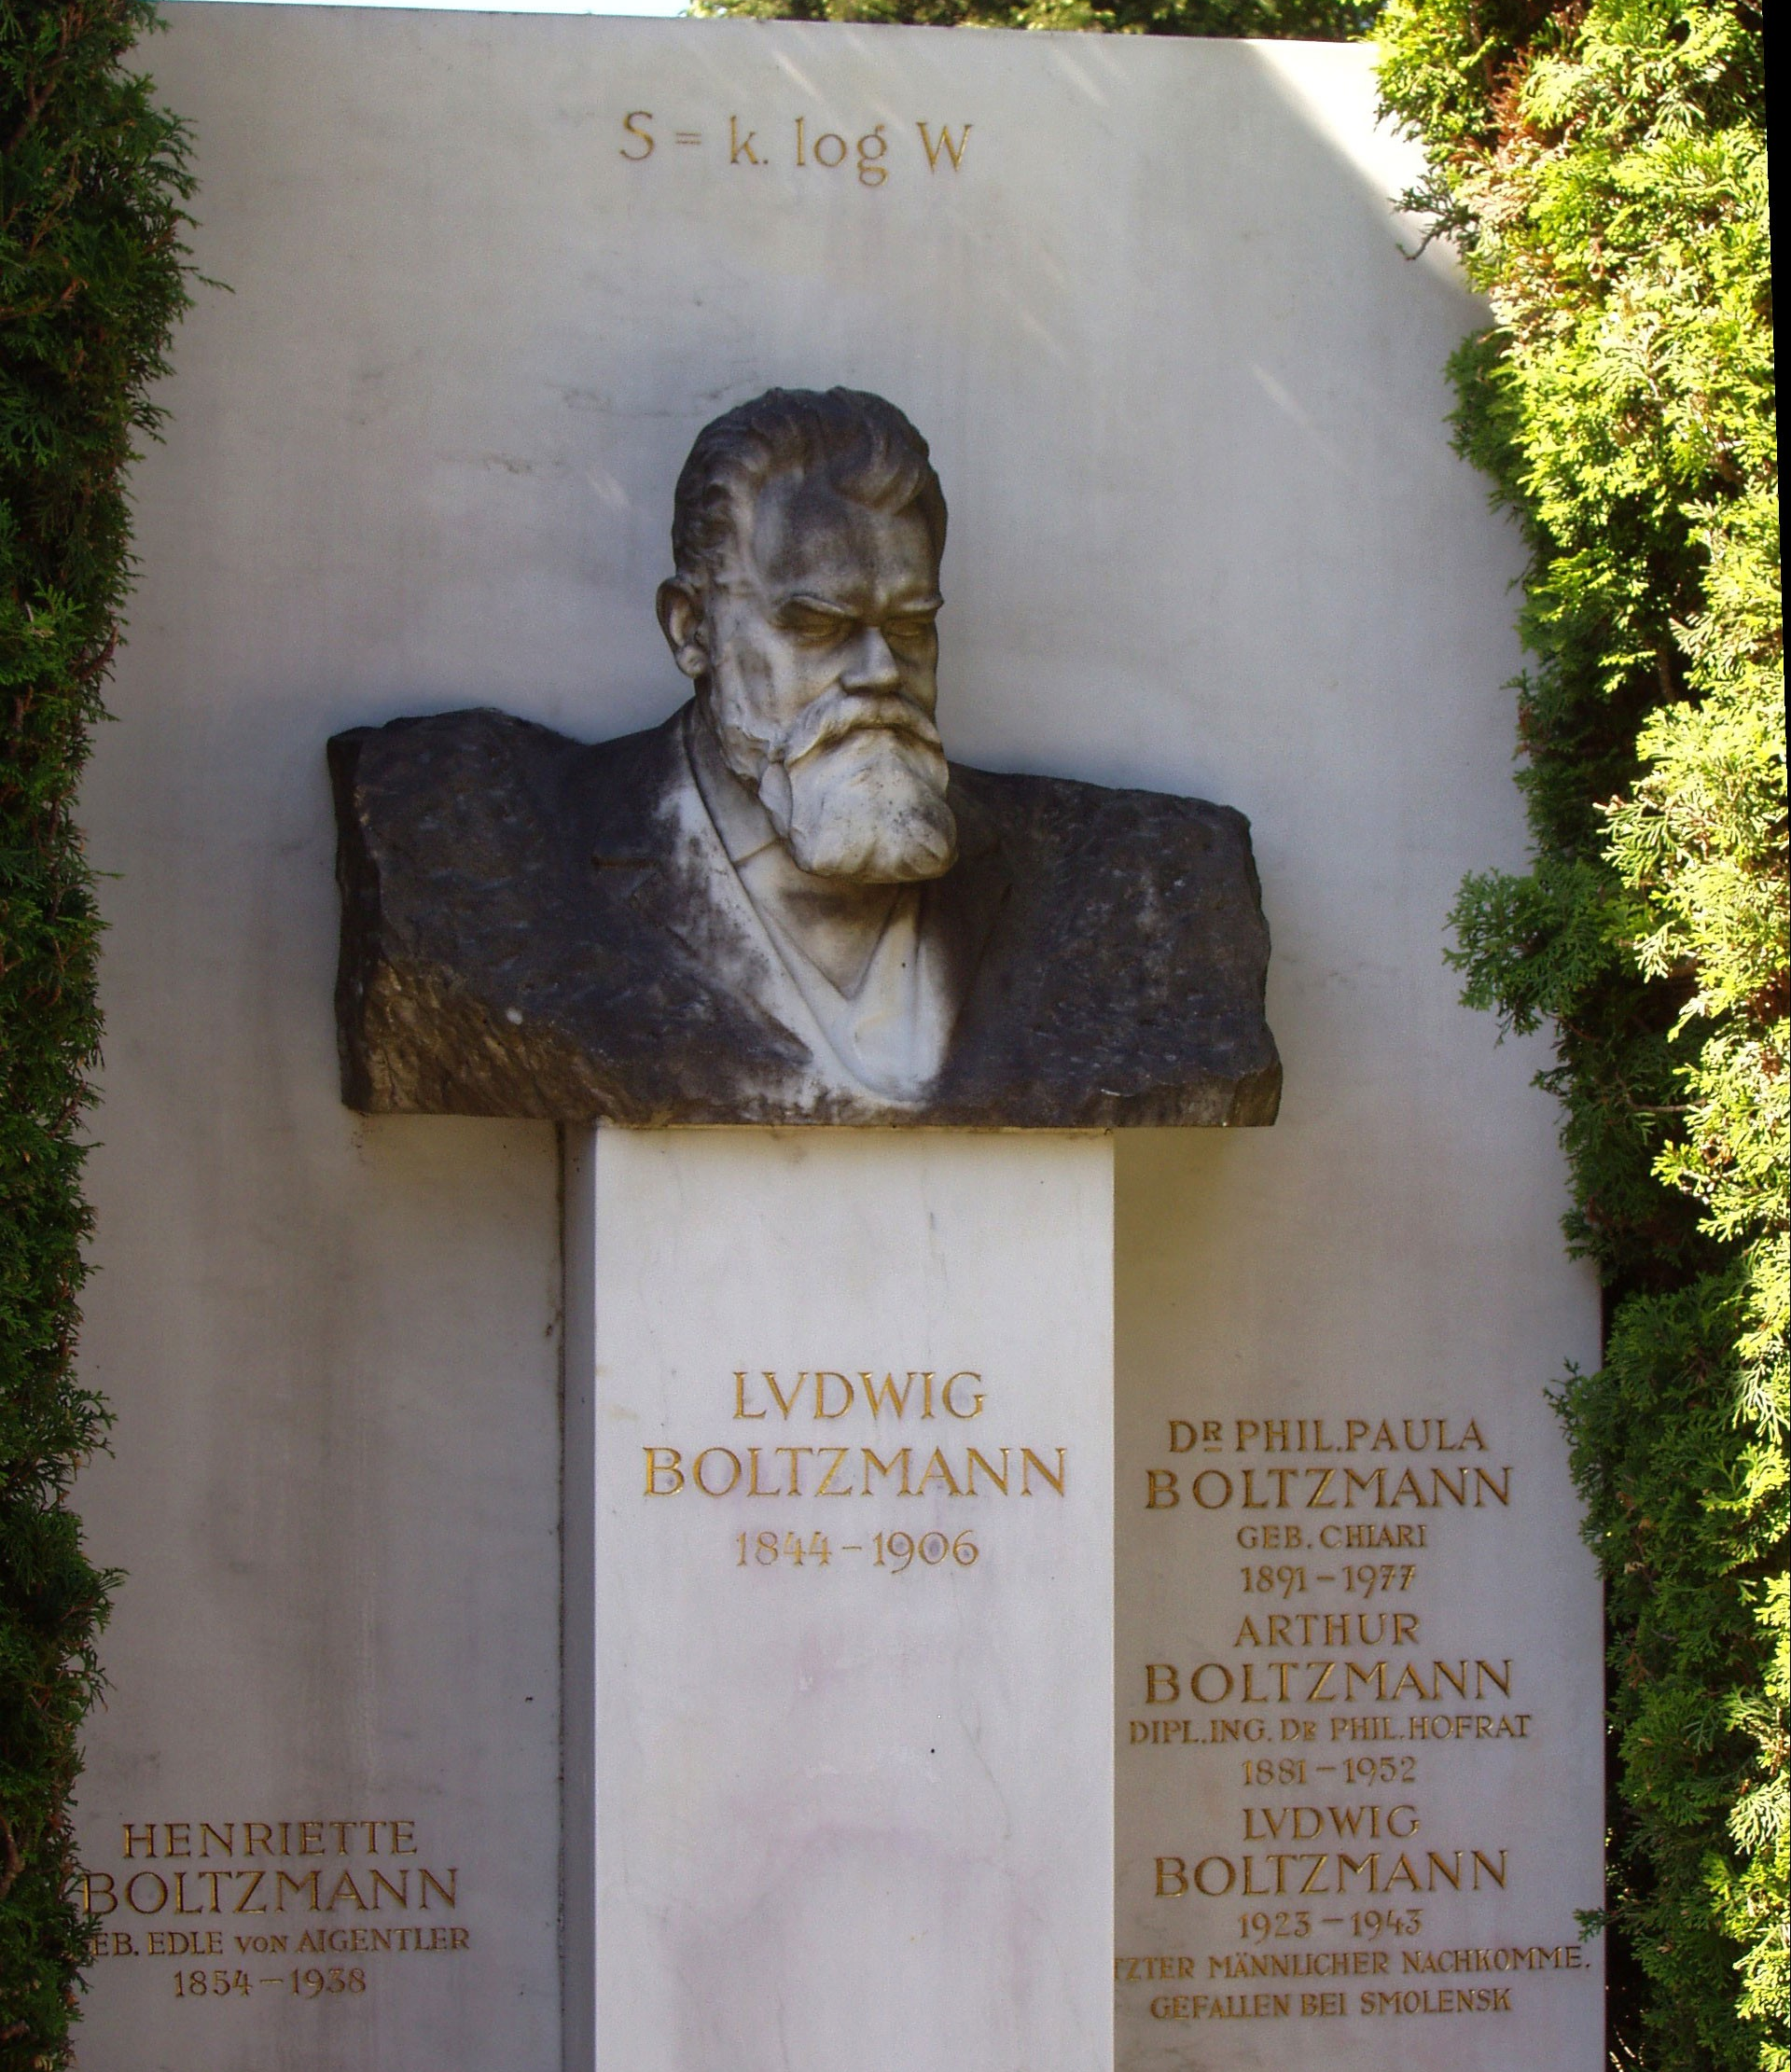
\includegraphics[height=0.6\textheight]{../img/boltzman.png}
				\caption{\label{fig:label} Tumba de Boltzman en Viena}
			\end{figure}

		\end{column}
	\end{columns}
\end{frame}

\begin{frame}
  \frametitle{Teoría Cinético Molecular (TCM)}
  \begin{columns}
    \begin{column}{0.5\textwidth}
      \begin{itemize}
        \footnotesize
        \item Una de las grandes conclusiones de LB es que para predecir el comportamiento de un gas podemos asumir que no poseen estructura interna. 
        \item Esto significa que podemos suponer el mismo comportamiento para un gas monoatómico, que para un gas poliatómico
        \item Esta sencilla, pero poderosa observación nos permite predecir un gas conocimiento muy pocos elementos de él.
        \item Actualmente sabemos que eso es cierto bajo ciertas condiciones $P \approx \qty{1}{atm}$ y $T < \qty{30}{\degreeCelsius}$
      \end{itemize}
    \end{column}
    \begin{column}{0.5\textwidth}
      \begin{figure}[ht]
        \centering
        \includegraphics[width=\textwidth]{../img/billar.jpg}
        \caption{El billar es un ejemplo de como se comporta microscópicamente todo gas ``ideal''}
        \label{fig:2}
      \end{figure}
    \end{column}
  \end{columns}
\end{frame}

\begin{frame}
  \frametitle{Variables de estado}
  \begin{columns}
    \begin{column}{0.5\textwidth}
      \begin{block}{Variable}
        Magnitud física que cambia. Ejemplo: tiempo.
        \begin{equation}
          \label{eq:1}
          f(x) \rightarrow x
        \end{equation}
      \end{block}
    \end{column}
    \begin{column}{0.5\textwidth}
      \begin{block}{Estado}
        Todas las variables que describen un sistema (gas).
        \begin{equation}
          \label{eq:2}
          E_{gas} = {r_1, r_2, r_3, r_3 ... r_n}
        \end{equation}
      \end{block}
    \end{column}
  \end{columns}
\end{frame}

\begin{frame}
  \frametitle{Variables y Unidades}
  \begin{columns}
    \begin{column}{0.5\textwidth}
      Las Variables que describen un gas ``ideal'' son:
      \begin{itemize}[<+->]
        \footnotesize
        \item Presión (P):Fuerza ejercida por unidad de área, sus unidades son: \unit{atm}, \unit{mmHg} o \unit{\pascal} (SI).
        \item Volumne (V): Espacio que ocupa un cuerpo (gas), sus unidades son: \unit{\liter} o \unit{\cubic\meter} (SI).
        \item Temperatura (T): Movimiento promedio de las partículas de un gas, sus unidades son: \unit{degreeCelsius}, \unit{\kelvin} (SI)
        \item Número de partículas (n), su unidad de medida es \unit{\mole} (SI)
      \end{itemize}
    \end{column}
    \begin{column}{0.5\textwidth}
      \begin{figure}[ht]
        \includegraphics<1>[width=\textwidth]{../img/presion.png}
        \only<1>{\caption{Presión}}
        \includegraphics<2>[width=\textwidth]{../img/volumen.png}
        \only<2>{\caption{Volumen}}
        \includegraphics<3>[height=0.6\textheight]{../img/temperature.jpg}
        \only<3>{\caption{Temperatura}}
        \includegraphics<4>[height=0.6\textheight]{../img/mole.jpg}
        \only<4>{\caption{Mol}}
      \end{figure}
    \end{column}
  \end{columns}
\end{frame}

\begin{frame}
  \frametitle{Sistema Internacional de Unidades (SI)}
  \begin{columns}
    \begin{column}{0.5\textwidth}
      \begin{itemize}
        \footnotesize
        \item Antiguamente para medir lo mismo se utilizaban diferentes medidas (ejemplo distancia: centimetros, codos, pulgadas, etc)
        \item Durante la revolución francesa se impuso la estandarización de medidas impulsando el sistema métrico por sobre otros.
        \item Actualmente es comúnmente aceptado usar las mismas unidades de medidas para las mismas magnitudes, existiendo dos grandes sistemas, el internacional (sistema métrico-decimal) y el anglosajón.
      \end{itemize}
    \end{column}
    \begin{column}{0.5\textwidth}
      \begin{figure}[ht]
        \includegraphics[width=0.6\textwidth]{../img/siu.png}
        \caption{Sistema Internacional de Unidades}
      \end{figure}
    \end{column}
  \end{columns}
\end{frame}

\section[Leyes de los gases]{Leyes de los gases: Boyle, Charles, Gay-Lussac y Avogadro}
\begin{frame}[allowdisplaybrakes]
  \frametitle{Ley de Boyle-Mariotte}
  \begin{columns}
    \begin{column}{0.5\textwidth}
      \begin{block}{}
        \justifying
        El británico-irlandés Robert Boyle (1627 - 1691) y el frances Edme Mariotte (1620 - 1684) en la década de 1670 descubren, independientemente, que la presión (P) por volumen (V) sin inversamente proporcionales, cuando la temperatura (T) y la cantidad de gas (n) son constantes.
        \begin{equation}
          \label{eq:3}
          P \propto \frac{1}{V}; T,n = cte
        \end{equation}
      \end{block}
    \end{column}
    \begin{column}{0.5\textwidth}
    \begin{figure}[ht]
      \includegraphics<1>[width=0.6\textwidth]{../img/boylemariotte.png}
      \only<1>{\caption{Robert Boyle y Edme Mariotte}}
      \includegraphics<2>[width=0.6\textwidth]{../img/boyle_law.png}
      \only<2>{\caption{Datos que muestran la relación inversa $k = PV$}}
    \end{figure}
    \end{column}
  \end{columns}

\end{frame}

\begin{frame}
  \frametitle{Ley de Charles}
  \begin{columns}
    \begin{column}{0.5\textwidth}
      \begin{definition}
        \justifying
        Jacques Charles, químico francés en la década de 1780 descubre que para un gas el volumen (V) y la temperatura (T) son directamente proporcionales, cuando la presión (P) y la cantidad de un gas (n) son constantes.
        \begin{equation}
          \label{eq:4}
          V \propto T; P,n = cte.
        \end{equation}
      \end{definition}
    \end{column}
    \begin{column}{0.5\textwidth}
      \begin{figure}[ht]
        \includegraphics<1>[width=0.5\textwidth]{../img/charles.jpg}
        \only<1>{\caption{Jacques Charles (1746 - 1823)}}
        \includegraphics<2>[width=\textwidth]{../img/charles_law.png}
        \only<2>{\caption{gráfico V y T}}
      \end{figure}
    \end{column}
  \end{columns}
\end{frame}

\begin{frame}
  \frametitle{Ley Gay-Lussac}
  \begin{columns}
    \begin{column}{0.5\textwidth}
      \begin{definition}
\justifying
        Joseph-Luis Gay-Lussac fue un químico francés que en la decada de 1808 cita los trabajos de Charles y una nueva relación: dónde la presión (P) y la temperatura (T) son proporcionales cuando el volumen (V) y la cantidad de gas (n) son constantes:
        \begin{equation}
          \label{eq:5}
          P \propto T; V,n = cte.
        \end{equation}
      \end{definition}
    \end{column}
    \begin{column}{0.5\textwidth}
      \begin{figure}[ht]
        \includegraphics<1>[width=0.5\textwidth]{../img/gaylussac.jpg}
        \only<1>{\caption{Joseph-Luis Gay-Lussac (1778 - 1850)}}
        \includegraphics<2>[width=0.6\textwidth]{../img/gaylussac_law.png}
        \only<2>{\caption{Gráfico de la Ley}}
      \end{figure}
    \end{column}
  \end{columns}
  
\end{frame}

\begin{frame}
  \frametitle{Ley de Avogadro}
  \begin{columns}
    \begin{column}{0.5\textwidth}
      \begin{definition}
\justifying
        Amadeo Avogrado científico y abogado italiano descubre en 1811 que el volumen (V) y la cantidad de gas (n) son proporcionales cuando la presión (P) y la temperatura (T) son constantes.
        \begin{equation}
          \label{eq:6}
          V \propto n; P,T = cte.
        \end{equation}
      \end{definition}
    \end{column}
    \begin{column}{0.5\textwidth}
      \begin{figure}[ht]
        \includegraphics<1>[width=0.6\textwidth]{../img/avogadro.jpg}
        \only<1>{\caption{Amadeo Avogrado (1776 - 1856)}}
        \includegraphics<2>[width=0.6\textwidth]{../img/avogadro_law.png}
        \only<2>{\caption{Gráfico de la ley}}
      \end{figure}
    \end{column}
  \end{columns}
\end{frame}

\begin{frame}
  \frametitle{Ecuación de estado de los gases ideales}
  \begin{columns}
    \begin{column}{0.5\textwidth}
      \begin{itemize}
        \item P [\unit{atm}]
        \item V [\unit{\litre}]
        \item n [\unit{\mole}]
        \item R = \qty{0,082}{atm.\litre\per\mole\kelvin}
      \end{itemize}
    \end{column}
    \begin{column}{0.5\textwidth}
      \begin{equation}
        \label{eq:7}
        PV = nRT
      \end{equation}
    \end{column}
  \end{columns}
\end{frame}

\begin{frame}
  \frametitle{Ejercicio}
\justifying
  Utilizando la \eqref{eq:7} resuelva el siguiente problema:
  \\\vspace{1cm}
  Si tenemos un \qty{1}{\mole} de gas a una presión de \qty{1}{atm} y \qty{0}{\degreeCelsius} ¿Cuál es su volumen? (Considere la ecuación $T_k = T_c + 273$ para convertir de celsius a kelvin)
\end{frame}

\begin{frame}
  \frametitle{Ley combinada de los gases ideales}
  \begin{columns}
    \begin{column}{0.5\textwidth}
\justifying
      Considerando todos los aportes realizados por los científicos anteriores es que se puede predecir cómo cambiará una variable de estado conociendo las otras, si la cantidad de gas se mantiene constante (n), entonces obtenemos:
    \end{column}
    \begin{column}{0.5\textwidth}
      \begin{equation}
        \label{eq:8}
        \frac{P_1V_1}{T_1} = \frac{P_2V_2}{T_2}
      \end{equation}
    \end{column}
  \end{columns}
\end{frame}

\begin{frame}
  \frametitle{Ejercicio}
\justifying
  Utilizando la \eqref{eq:7} responda:
  \\\vspace{0.5cm}
  Una gas ocupa un volumen de \qty{80}{\cubic\centi\metre} a una presión de \qty{750}{mmHg}. ¿Qué volumen ocupará a una presión de \qty{1.2}{atm} si la temperatura no cambia? (\qty{1}{cc} = \qty{1}{\milli\litre} y \qty{1}{atm} = \qty{760}{mmHg})
\end{frame}

\section{Aplicación de la Ley de los gases ideales}

\begin{frame}
  \frametitle{El despliegue de los Airbags en milisegundos}
  \begin{columns}
    \begin{column}{0.5\textwidth}
      \footnotesize
      Es quizás la aplicación más crítica para salvar vidas. Cuando un sensor detecta una colisión, se activa una reacción química que genera gas nitrógeno (\ce{N2}​) de forma instantánea.
  \begin{itemize}
    \item \textbf{Química detrás}: Para que el airbag te proteja, debe pasar de un estado sólido (pequeño volumen) a un gas que llene la bolsa (gran volumen) en unos 30 a 50 \unit{\milli\seconds}.
    \item \textbf{Relación}: Al aumentar drásticamente el número de moles (n) de gas dentro de la bolsa, el volumen (V) se expande violentamente para mantener el equilibrio, incluso si la presión externa es constante.
  \end{itemize}
\end{column}
\begin{column}{0.5\textwidth}
  \begin{figure}[ht]
   \includegraphics[width=0.6\textwidth]{../img/airbag.jpg}
  \end{figure}
\end{column}
\end{columns}
\end{frame}

\begin{frame}
  \frametitle{Problema: El AirBag}
  Un airbag de conductor tiene un volumen de \qty{60}{\litre}. Para que sea efectivo, debe inflarse a una presión de \qty{1.2}{atm} a una temperatura de \qty{25}{\degreeCelsius}. ¿Cuántos moles de gas Nitrógeno (\ce{N2}​) deben producirse instantáneamente?
\end{frame}

\begin{frame}
  \frametitle{Exploración Espacial: SpaceX y los tanques de combustible}
  \begin{columns}
    \begin{column}{0.5\textwidth}
\footnotesize
  En cohetes como el Starship, el manejo de los gases es una obra de arte de la ingeniería. Utilizan metano y oxígeno líquidos, pero estos deben mantenerse a presiones y temperaturas muy específicas.
  \begin{itemize}
    \item \textbf{La química detrás}: Cuando los ingenieros "presurizan" los tanques para empujar el combustible hacia los motores, utilizan gases como el helio.
    \item \textbf{Relación}: Si la temperatura (T) en el espacio cambia drásticamente al recibir luz solar, la presión (P) dentro de los tanques de fibra de carbono podría aumentar hasta niveles peligrosos si no se controla el volumen o se libera masa (n).
  \end{itemize}
    \end{column}
    \begin{column}{0.5\textwidth}
      \begin{figure}[ht]
        \includegraphics[width=0.6\textwidth]{../img/spacex.jpg}
      \end{figure}
    \end{column}
  \end{columns}
\end{frame}

\begin{frame}
  \frametitle{Problema: Tanques de SpaceX}
  Un tanque de Helio para presurización en un cohete está a \qty{200}{atm} cuando la temperatura en la plataforma de lanzamiento es de \qty{20}{\degreeCelsius}. Si en el espacio, debido a la radiación solar, la temperatura del tanque sube a \qty{80}{\degreeCelsius}, ¿cuál será la nueva presión interna? (Asume volumen constante).
\end{frame}

\begin{frame}
  \frametitle{Buceo de alta profundidad y ``las burbujas en la sangre''}
  \begin{columns}
    \begin{column}{0.5\textwidth}
\footnotesize
  Si alguna vez te has preguntado por qué los buceadores no pueden subir rápido a la superficie, la respuesta está en $PV=nRT$.
  \begin{itemize}
    \item \textbf{La química detrás}: A medida que un buzo desciende, la presión (P) aumenta. Según la ley, si la presión sube, el volumen (V) de los gases disminuye. El nitrógeno del aire comprimido se disuelve en la sangre debido a esa alta presión.
    \item \textbf{El peligro}: Si el buzo sube demasiado rápido, la presión (P) cae bruscamente y el nitrógeno vuelve a su estado gaseoso rápidamente, creando burbujas en el torrente sanguíneo (como cuando abres una soda agitada).
  \end{itemize}
    \end{column}
    \begin{column}{0.5\textwidth}
      \begin{figure}[ht]
        \includegraphics[width=\textwidth]{../img/divebubble.png}
      \end{figure}
    \end{column}
  \end{columns}

\end{frame}

\begin{frame}
  \frametitle{Problema: Buceo Profundo}
\justifying
  Un buceador a \qty{30}{\metre} de profundidad exhala una burbuja de aire de \qty{10}{\milli\litre}. A esa profundidad, la presión es de \qty{4}{ atm}. ¿Qué volumen tendrá esa burbuja cuando llegue a la superficie, donde la presión es de 1 atm? (Asume temperatura constante).
\end{frame}

\begin{frame}
  \frametitle{Ventiladores Médicos (Cuidados Intensivos)}
  \begin{columns}
    \begin{column}{0.5\textwidth}
\footnotesize
      Durante la pandemia de COVID-19, los ventiladores se volvieron protagonistas. Estos dispositivos son básicamente computadoras que aplican las leyes de los gases con precisión quirúrgica.
      \begin{itemize}
        \item \textbf{La química detrás}: El pulmón humano tiene un límite de presión que puede soportar antes de sufrir un daño (barotrauma).
        \item \textbf{Relación}: El ventilador calcula exactamente cuánto volumen (V) de aire oxigenado debe introducir basándose en la temperatura corporal (T) y la resistencia de los pulmones, asegurando que la presión (P) nunca exceda los límites de seguridad.
      \end{itemize}
    \end{column}
    \begin{column}{0.5\textwidth}
      \includegraphics[width=\textwidth]{../img/mechvent.jpg}
    \end{column}
  \end{columns}
\end{frame}

\begin{frame}
  \frametitle{Problema: Ventilador Médico}
\justifying
  Un ventilador introduce \qty{500}{\milli\litre} de aire en los pulmones de un paciente. El aire está en el equipo a temperatura ambiente (\qty{20}{\degreeCelsius}). Al entrar a los pulmones, el aire se calienta a la temperatura corporal (\qty{37}{\degreeCelsius}). Si la presión se mantiene constante, ¿cuál es el volumen final del aire dentro del pulmón?
\end{frame}

\begin{frame}
  \frametitle{El funcionamiento de las Ollas a Presión}
  \begin{columns}
    \begin{column}{0.5\textwidth}
\footnotesize
    Un clásico moderno en la cocina. ¿Por qué la comida se cocina más rápido?
    \begin{itemize}
      \item \textbf{La química detrás}: Al calentar el agua en un recipiente cerrado, el volumen (V) es constante.
      \item \textbf{Relación}: Al aumentar la temperatura (T), la presión (P) sube significativamente. Esta alta presión eleva el punto de ebullición del agua por encima de los \qty{100}{\degreeCelsius}, permitiendo que los alimentos se cocinen a temperaturas mucho más altas sin que el agua se evapore, reduciendo el tiempo de cocción a la mitad.
    \end{itemize}
    \end{column}
    \begin{column}{0.5\textwidth}
      \includegraphics[width=\textwidth]{../img/instantpot.jpg}
    \end{column}
  \end{columns}
\end{frame}

\begin{frame}
  \frametitle{Problema: Olla de Presión (Límite de seguridad)}
  \justifying
  Una olla de presión contiene aire y vapor a \qty{1}{atm} y \qty{20}{\degreeCelsius}. La válvula de seguridad está diseñada para dispararse cuando la presión llega a \qty{2.5}{atm}. ¿A qué temperatura empezará a liberar vapor la olla?
\end{frame}


\section{Cálculos estequimétricos en gases ideales}

\begin{frame}
  \frametitle{Bibliografía}
  \begin{thebibliography}{99}
    \setbeamertemplate{bibliography item}[book]
    \bibitem[Chang, 2011]{Chang2011}
    Chang, Raymond
    \newblock \emph{Fundamentos de Química}
  \end{thebibliography}
\end{frame}



\end{document}
